
\section{Uniform Bundle and Item Pricing}

In this section, we provide some worst-case guarantees on how well uniform bundle pricing and item pricing can approximate the 
optimal subadditive and monotone bundle pricing. 


\begin{figure}[t]
	\scalebox{.95}{
		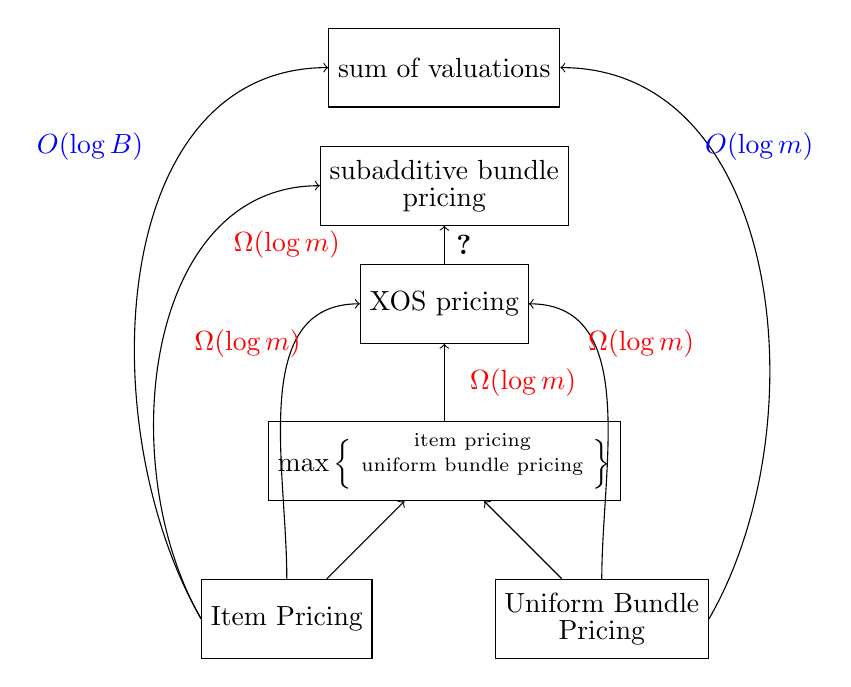
\begin{tikzpicture}
		\node (rectsum) [rectangle, draw, minimum width=7mm, minimum height=10mm] at (0,1.5) {sum of valuations};
		
		\node (rectbundle) [rectangle, draw, minimum width=7mm, minimum height=10mm] at (0,0) {\shortstack{subadditive bundle \\ pricing}};
		
		\node (rectxos) [rectangle, draw, minimum width=7mm, minimum height=10mm] at (0,-1.5) {XOS pricing};
		
		\node (rectmax) [rectangle, draw, minimum width=7mm, minimum height=10mm] at (0,-3.5) {$\max \Big\{$  \shortstack{\scriptsize item pricing \\ \scriptsize uniform bundle pricing} $\Big\}$};
		
		\node (rectitem) [rectangle, draw, minimum width=7mm, minimum height=10mm] at (-2,-5.5) {Item Pricing};
		
		\node (rectubundle) [rectangle, draw, minimum width=7mm, minimum height=10mm] at (2,-5.5) {\shortstack{Uniform Bundle \\ Pricing}};
		
		\draw [->] (rectubundle.east) to [out=60, in = 0] (rectsum);
		\node at (4,0.5) {\textcolor{blue}{$O( \log m)$}};
		\draw [->] (rectubundle) to [out=90, in = 0] (rectxos);
		\node at (2.5,-2) {\textcolor{red}{$\Omega( \log m)$}};
		\draw [->] (rectitem.west) to [out=120, in = -180] (rectsum.west);
		\node at (-4.5,0.5) {\textcolor{blue}{$O( \log B)$}};
		\draw [->] (rectitem) to [out=90, in = -180] (rectxos.west);
		\node at (-2.5,-2) {\textcolor{red}{$\Omega( \log m)$}};
		\draw [->] (rectxos) to  (rectbundle);
		\node at (0.25,-0.75) {\textbf{?}};
		\draw [->] (rectitem.west) [out = 120, in = -180] to  (rectbundle.west);
		\draw [->] (rectmax)  to  (rectxos);
		\draw [->] (rectitem)  to  (rectmax);
		\draw [->] (rectubundle)  to  (rectmax);		
		\node at (-2,-0.75) {\textcolor{red}{$\Omega( \log m)$}};
		\node at (1,-2.5) {\textcolor{red}{$\Omega( \log m)$}};
		
		\end{tikzpicture}
	}
	\caption{Results Summary: Red font show results in this paper; blue font shows existing known results}
	\label{fig:summary}
\end{figure}

\paragraph{Upper Bounds.}
It is a folklore result that for any hypergraph $\mH = (\mV, \mE)$ with valuations $\{v_e\}_{e \in \mE}$, one can always construct a uniform bundle price that is $O(\log m)$ away from
the sum of valuations $\sum_e v_e$, which is an upper bound on the optimal subadditive and monotone bundle pricing (for completeness, we provide a proof in Appendix~\ref{sec:appendix}). Similarly, we know from~\cite{cheung2008approximation} that item pricing can achieve a $O(\log B)$ approximation of the sum of valuations. Recall that 
$B$ is the maximum number of hyperedges that a vertex can be contained in, and hence $B \leq m$. 

\paragraph{Lower Bounds.}
The upper bound of $O(\log m)$ is tight in the worst case for both uniform item pricing and bundle pricing. In particular, we show the following stronger results:
%
\begin{enumerate}
\item There exists a hypergraph instance with additive valuations where any uniform bundle price produces revenue that is $\Omega(\log m)$ away from the optimal (Lemma~\ref{lem:lb1} in the appendix).
\item There exists a hypergraph instance with uniform valuations (\ie, each buyer has the same valuation for any hyperedge) where any item pricing produces revenue that is $\Omega(\log m)$ away from the optimal (Lemma~\ref{lem:lb2} in the appendix).
\item There exists a hypergraph instance with submodular valuations where any item pricing {\em and} any uniform bundle pricing is  $\Omega(\log m)$ away from the optimal (Lemma~\ref{lem:lb3} in the appendix).
\end{enumerate} 
 



